\chapter{Experiment 1: game session with provoved stress and boredom}

\section{Introduction}

, however its reliability within a context involving natural behavior must be checked. The methods are sensitive to noise caused by movement, facial expressions or changes in illumination (e.g. screen activity reflected on user's face), which are all likely to happen in such sessions with natural behavior. Those interferences might produce unreliable measurements of the HR signal, resulting in misleading investigations. It is important to establish the reliability of remote HR measurements under situations with natural behavior, where users are not instructed to behave differently than what they usually do. In that light this paper presents an analysis of the remotely obtained HR signal of users within such natural context. We developed a set of casual-themed, similar to off-the-shelf games that were carefully designed to present stressful and boring moments, which should induce players to present variations of HR. During the gaming sessions, the player's HR signal was remotely estimated using the work by \textcite{poh2011advancements}, an established rPPG technique for HR estimation. A physical sensor was used as ground truth. A comparison and analysis of the accuracy of remote HR estimations are presented and discussed. The main contribution of this paper is the accuracy evaluation of an established rPPG technique within the context of gaming sessions where users behave naturally instead of following movement constraint rules, e.g. remain still. Our results provide researchers with information related to the reliability of a remote HR measurement technique when applied to contexts where users behave more naturally

The use of remote measurement of physiological signals, such as rPPG, has already been applied to emotion detection. Signals as HR and HRV were used to remotely detect stress \parencite{mcduffcogcam, mcduff2014improvements, bousefsaf2013remote}, for instance. Since the estimations of rPPG techniques are significantly affected by external noise, e.g. subject's movement, experimental results are usually accompanied by accuracy evaluations regarding the estimations of the employed rPPG technique. In the majority of the cases, subjects are typically instructed to stay still \parencite{rouast2016remote}, which improves the accuracy of the rPPG technique. In some other cases, however, authors evaluate the accuracy of the HR estimation under scenarios where subjects are instructed to act naturally. Despite the fact that such works present experiments where subjects are told to behave naturally, their accuracy evaluation is based on artificial or simple human-computer interactions. Subjects are idly staring at the camera \parencite{zhao2013remote,hsu2014learning}, faking an interaction with a computer \parencite{poh2010non}, working on a task, i.e. make a website \parencite{monkaresi2014machine} or mentally subtract numbers \parencite{mcduff2014remote}, or performing arbitrary movements \parencite{tran2015robust}, e.g. head rotation in different degrees.

Another important factor is the material used to produce the emotional stimuli. Subjects are not interacting with a complete digital game in any of the experiments, which hinders the accuracy evaluation of rPPG techniques within the context of games research, for instance. Authors commonly use images, videos or text as content to produce the emotional stimuli. When game-like materials are used, however, they are often gamified cognitive tests, e.g. Stroop test \parencite{golden1978stroop}. Additionally the experiment duration varies from 20 seconds to 10 minutes and the non-game stimuli content is less likely to produce the reactions of a real gaming session, for instance spontaneous body movement and facial actions.

In that context, we designed and carried out an experiment focused on the accuracy evaluation of an rPPG technique applied to real gaming sessions, using custom made games as emotion stimuli. Our experiment is based on the previously mentioned findings that HR varies according to stress/frustration and that facial expressions can convey contextual information about emotional state \parencite{giannakakis2017stress}. As opposed to those previously mentioned works, in our experiment each subject spends an average of 25 minutes in the session, playing three different games that were custom-made to provoke the emotional reactions similar to off-the-shelf games. Subjects were also not instructed regarding how they should move, so body and facial reactions are likely to be the ones the subject would normally perform under a gaming context. Our approach consists of using induced boring to stressful mechanics in the games to produce variations in the emotional state and HR of participants, based on the previously mentioned findings that HR varies according to stress/frustrations. We aim to explore the accuracy of rPPG-estimated HR readings of subjects while playing under such circumstances. To the best of our knowledge, this is the first experiment to measure the accuracy of an rPPG technique with the use of three boredom/stress-inducing games with subjects behaving naturally.

%The remote detection of HR proved a promising approach to infer boredom/stress levels \parencite{kukolja2014comparative} or cognitive stress \parencite{mcduff2014remote} of a person. Experiments regarding such approaches, however, were performed under extremely controlled situations with few game-related stimuli. A significant limitation of such approaches was that subjects were asked to remain still during the experiment. Another problem is that subjects had limited interaction with the content being presented: they performed tasks mentally (e.g. counting), watched videos/images or performed gamified cognitive tests for a short period of time. Those are artificial situations that are unlikely to happen in real-life situations, especially in a gaming session with a challenging game lasting for several minutes. In that situation, the subject will probably move and present variations of facial actions during the gaming session \parencite{bevilacqua2016variations}.

%%%%

In order to explore the relation among facial actions, HR and emotional states, particularly stress and boredom, we designed and carried out an experiment involving games that were deliberately designed to cause the aforementioned emotional states. Our approach consists of recording participants while they play three different games that were carefully designed and developed to have a very similar difficulty balance that linearly progresses from a boring to a stressful state. Our experiment has two main goals. The first one is to measure the variations of the HR mean to test the hypothesis that the mean of the differences of HR during boring and stressful parts of the games is different. The second goal is to empirically explore how facial actions (FA), defined by us as being any facial movement different from a neutral face, e.g. lips contraction, manually detected and annotated with observations, relate to emotional states. Our experiment allows the investigation of variations of HR and FA in a context where boredom and stress were induced on purpose. As a result of our experiment, we present information regarding the changes in the HR mean of subjects while they play games that are deliberately boring and stressful; additionally we present a set of annotated FA that happened during the phases of the games that were perceived as being boring and stressful. Our main contribution is twofold: firstly we introduce information about the variations of HR that occurred during the interaction with the games, specially under situations that were designed to provoke boredom and stress. Our results indicate with statistical significance that the HR mean is different during boring and stressful situations in our games. Secondly we present information regarding the frequency which the annotations of naked-eye recognizable FA happened during specific phases of the games, all obtained from the analysis of about 6 hours of recordings from 20 subjects. We include an analysis and discussion of the gathered information. We believe that this paper contributes with information regarding HR and FA in the context of games, which can be combined to create user-tailored models for emotion detection based on different data sources. Additionally we highlight the heterogeneous nature of our group of subjects that have significantly different ages and gaming experiences, which produces a diverse sample for the investigation of changes in HR, FA and emotional states. In the remainder of this paper we will: summarize related works regarding the mapping of facial and physiological signals to emotional states; explain our experiment; show and discuss the results; finally we present a conclusion.


\section{Participants, materials and procedures}

Twenty adult participants of both genders (10 female) with different ages (22 to 59, mean 35.4, SD 10.79) and different gaming experience gave their informed and written consent to participate in the experiment. The study population consisted of staff members and students of the University of Sk\"ovde, as well as citizens of the community/city. When asked how skilled subjects believe they are at playing video games, 1 subject (5\%) reported no skill, 10 (50\%) reported not very skilled, 7 (35\%) reported moderately skilled and 2 (10\%) reported very skilled. When asked the number of hours per week they had played any type of video game over the last year, 2 subjects (10\%) reported more than 10, 6 (30\%) reported 5 to 10, 2 (10\%) reported 3 to 4, 2 (10\%) reported 1 to 3, 4 (20\%) reported 0 to 1, and 4 (20\%) reported no activity. Those numbers indicate that our population has a diversity of gaming experience and playing frequency, which provides us with information that is less skewed towards specific profile of players, e.g. hardcore players. Subjects were seated in front a computer, alone in the room, while being recorded by a camera and measured by a heart rate sensor. The camera was attached to a tripod placed in front of the subjects at approximately 0.6m of distance; the camera was slightly tilted up. A spotlight, tilted 45$^{\circ}$ up, placed at a distance of 1.6m from the subject and 45cm higher than the camera level, was used for illumination; no other light source was active during the experiment. Figure \ref{fig:setup} illustrates the setup.

\begin{figure}
\centering
\includegraphics[width=\textwidth]{figures/experiment-setup-double}
\caption{Experiment setup. On the left, illustration regarding the position of equipment, including the angle of the external light source. On the right, highlight of the position and angle of the video camera.}
\label{fig:setup}
\end{figure}

The participants were each recorded for about 25 minutes, during which they played three games. Each game was followed by a questionnaire related to the game and stress/boredom. The first two games were followed by a 138 seconds rest period, where the subjects listened to calm classic music. The last game was followed by an additional questionnaire about age and gaming experience/profile. The order which the games were played was randomized among subjects. Participants received instructions from a researcher that they should play three games, answer a questionnaire after each game and rest; they were told that their gaming performance was not being analyzed, that they should not give up in the middle of the games and that they should remain seated during the whole process.

During the whole experiment, subjects were recorded using a Canon Legria HF R606 video camera. All videos were recorded in color (24-bit RGB with three channels $\times$ 8bits/channel) at 50p frames per second (fps) with pixel resolution of 1920 $\times$ 1080 and saved in AVCHD-HD format, MPEG-4 AVC as the codec. At the same time, subject's HR was measured by a TomTom Runner Cardio watch (TomTom International BV, Amsterdam, Netherlands), which was used as ground truth. The watch was placed on the left arm, approximately 7cm away from the wrist, like a regular wrist watch, and its use was unobtrusive, so it did not affect the movements of the subjects, who could still use both hands to play the games. The watch recorded the HR at 1 Hz.

\subsection{Questionnaires}

After each game, subjects answered a questionnaire in order to provide self-reported stress and bordeom measurements. The questionnaire had six questions: the first four were a 5-point Likert scale related to how the player felt related to stress/boredom at the beginning/end of each game (1: not stressed/bored at all, 5: extremely stressed/bored); a question to identify the part of the game that best describes the moment the subject enjoyed the most (very beginning, after beginning and before middle, middle, after middle and before end, very end); finally a question asking if the subject understood the game. Before the end of the experiment, subjects answered a final questionnaire with nine questions, which were related to: age; gender; number of hours per week spent with games over the last year (question from the video game experience questionnaire \parencite{unsworth2015playing}); how proficient or skilled the subject believe being at playing video games (question from the Survey of Spatial Representation and Activities - SSRA \parencite{terlecki2005important}); familiarity with puzzle, platform and Tetris games; current state of mind compared to other days (e.g. normal, unusually stressed, etc.); and gaming profile (like, dislike challenging games).

\section{Games and stimuli elicitation}

The three games\footnote{Source code available at: https://github.com/Dovyski/face-tracking-games} used in the experiment were 2D and casual-themed, played with mouse or keyboard in a web browser. The games were carefully designed to provoke boredom at the beginning and stress at the end, with a linear progression between the two states (adjustments of such progression are performed every 1 minute). The game mechanics were chosen based on the capacity to fulfill such linear progression, along with the quality of not allowing the player to instantly kill the main character (by mistake or not), e.g. by falling into a hole. The mechanics were also designed/selected to ensure that all subjects would have the same game pace, e.g. a player must not be able to deliberately control the game speed based on his/her will or skill level.

The \textbf{Mushroom} game, illustrated in Figure \ref{fig:mushroom-platformer-tetris} (left), is a puzzle where the player must feed a character by dragging and dropping mushrooms in rounds. In a given round, $M$ mushrooms are displayed in a grid and the player has $K$ seconds (a decreasing time bar at the top informs the remaining time) to collect good and discard bad (poisonous) mushrooms. At the upper-right corner of the screen, a sign informs the player about the bad/poisonous mushroom of the round. The player must drag and drop all good mushrooms (the ones different from the poisonous indication) into the character, while dragging and dropping the bad ones into the trash can. Mushrooms are differentiated by the colors of their features (circles). The player is rewarded with score points, a health bar increase ($HB\textsubscript{I}$) and a pleasant sound when a right move is performed. In case of mistake a health bar decrease ($HB\textsubscript{D}$) and an annoying/aggressive alarm sound is applied. If the time $K$ is over and the player has not finished moving all the mushroom of the round, each remaining mushroom in the grid is counted as a mistake. If the grid is clean and there is still time available, the player must wait until the time is over. The values of $M$, $K$, $HB\textsubscript{I}$ and $HB\textsubscript{D}$ are used to induce boredom/stress. At the beginning, $M$ is low (starts with 2) and $K$ is high (starts with 45 seconds), so the player spends a significant amount of time waiting for the game to continue; every 1 minute the value of $M$ is increased and $K$ is decreased. The changes continue to happen until the player is unable to deal with the amount of mushrooms within the available time. This leads to mistakes that will eventually decrease the health bar to zero, terminating the game. After the mark of 6 minutes, the game becomes virtually impossible to beat.

The \textbf{Platformer}, illustrated in Figure \ref{fig:mushroom-platformer-tetris} (center), is a side-scrolling, endless runner game where the player must control the main character while collecting hearts and avoiding obstacles (skulls with spikes). The character can jump (by pressing the up arrow key in the keyboard) or slash (S key), however the player is not able to move the main character left or right, it remains in the same position on the screen (towards the left side of the screen). The character moves on top of platforms, which are always perfectly connected, so there are no gaps (holes) among them; the height of the platform can vary, however, so there might be a slope up/down connecting two platforms, for instance. If the character hits an obstacle, the health bar is decreased ($HB\textsubscript{D}$) and a sound effect related to pain is played. If any heart is collected, the health bar increases ($HB\textsubscript{I}$) and a pleasant sound effect is played. The position where the hearts appear on each platform is adjustable (defined by $HH$), so they can appear close to the platform (no action is required to collect the heart) or a bit higher from the ground (jump action is required to collect the heart). The speed of the character ($S$, which is the velocity at which elements are moving on the screen), the height variation of each new platform that appears on the screen ($HV$), the amount of hearts ($G$) and obstacles ($E$) per platform are all controlled by the game and used to adjust boredom/stress. At the beginning, boredom is induced by keeping all previously mentioned parameters with low values, which means the game is slow, the character moves from platform to platform at the same height and almost no hearts or obstacles appear on the screen. The few hearts that are available are placed close to the ground to destimulate jumping actions. As time progresses, the values of $S$, $E$, $HV$, $HB\textsubscript{D}$ and $HH$ increase, while $G$ and $HB\textsubscript{I}$ decrease to induce the player to a stressfull state. At the mark of 5 minutes, for instance, the game is significantly fast, with several obstacles on the screen and almost no hearts to collect; the damage caused to the character when hit by an obstacle is also higher than the beginning of the game. The linear increase in difficulty will eventually result in consecutive hits (mistakes), which will decrease the health points until zero, when the game ends.

\begin{figure*}[!t]
\centering
\includegraphics[width=\textwidth]{figures/experiment1-games}
\caption{Mushroom (left), Platformer (center) and Tetris (right). In Mushroom, player has to drag and drop the correct mushrooms into the character, discarding the wrong ones into the trash. In Platformer, the player has to jump over or slide under obstacles while collecting hearts. In our version of Tetris, there are no hints about the next piece to be added to the screen}
\label{fig:mushroom-platformer-tetris}
\end{figure*}

Finally the game \textbf{Tetris}, shown in Figure \ref{fig:mushroom-platformer-tetris} (right), is a modification of the original Tetris game. In our version of the game, the next block to be added to the screen is not displayed, so the player is unable to predict future moves. Additionally, the down key, usually used to speed up the descendant trajectory of the current piece, is disabled. The keyboard controls are the arrow keys to move the piece left/right and the R key to rotate the piece. The game is also modified to ensure that all subjects received the same sequence of pieces (we use the same seed for the generation of random numbers). The speed that the pieces fall ($S$) is used to control boredom and stress; at the beginning of the game, boredom is induced by using a low value for $S$, which makes the game slow since the pieces are falling slowly and the player is unable to speed them up. As time progresses, $S$ increases linearly making the game faster and harder to play, which should induce stress. At the mark of 5 minutes, for instance, a single piece takes almost 1 second to traverse the whole screen.

\section{Study 1: variations of facial actions}

This study presents information regarding FA that the subjects presented during the experiment. The 6 hours of recordings of all subjects were manually analyzed and FA were annotated empirically. The annotations were categorized according to the period when they happened (the boring first part or the stressful second part of the games). An analysis on such annotated FA was conducted on group and individual level, aiming to find patterns between the featured FA and the boring/stressful periods of the games.

The following sections presents the analysis, discussion and results of the gathered information.

\subsection{Analysis and methods}
\label{s:experiment1-study1-methodology}

The recordings of all subjects were analyzed by a single reseacher who took notes of any facial actions (FA) that were different from a neutral (resting) face, e.g. lips contraction, brow movement, etc. Annotations were not performed periodically, e.g. every 5 seconds, instead they were made only when the subject's face changed from its neutral/resting state. As a consequence, if the subject remained with a neutral face for a long period of time, no annotations were made during that period.

The use of such empirical and non-standard approach for facial annotation was used because focus is not on facial expressions \textit{per se}, but in the exploration of any facial action (standardized or not) that might be used to infer patterns in boredom/stressful states. This approach is not without its limitations, however it provides a reasonable empirical perception of facial activity that is different from a neutral face, which is satisfactory for the investigation. FA are subtle and not necessarily part of a complete facial expression, e.g. surprise face, so they might be better identified in a context where annotations are made only when facial changes happen, as opposed to a frame-by-frame analysis/annotation of a video, for instance.

\begin{figure}[!h]
\centering
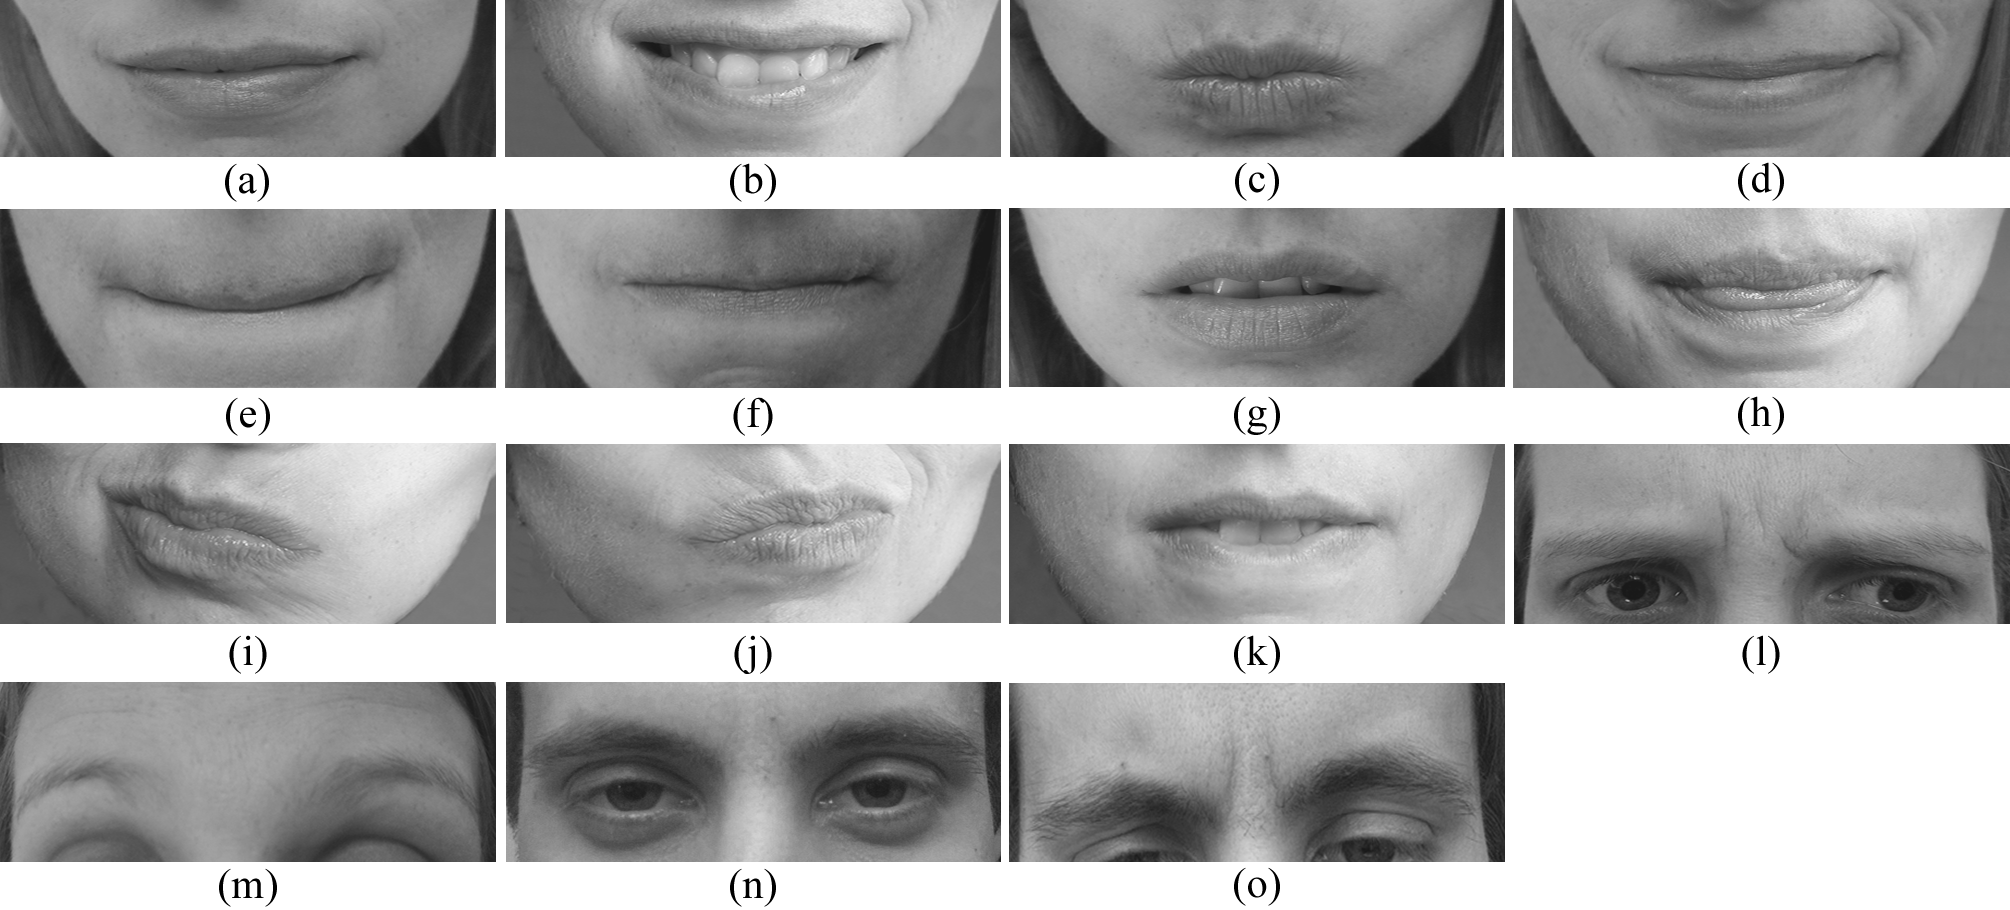
\includegraphics[width=0.4\textwidth]{figures/facial-actions}
\caption{Annotated facial actions (FA). (a) Smile not showing teeth; (b) Smile showing teeth; (c) Lip puckerer; (d) Lip stretcher; (e) Lip suck; (f) Lip pressor; (g) Lips parted; (h) Tongue touching lips; (i) Mouth movement right; (j) Mouth movement left; (k) Lower lip bite; (l) Frown; (m) Brow raiser; (n) Lid tightener; (o) Brow lowering}
\label{fig:fa}
\end{figure}

According to the design of the games, subjects are supposed to perceive the experience during the beginning of the games as being more boring than the one at the end, while the experience at the end should be perceived as more stressing than the one at the beginning of the games. As a result, if the game sessions of each subject is divided in half, in theory one of the two resulting parts is more likely to be perceived as more boring by the subjects, while the other is more likely to be perceived as more stressful. Using that assumption, FA annotations were divided in two groups, the ones made during the period that corresponds to the first half ($H_0$) of the games and the ones made in the second half ($H_1$). Such division of the annotation aimed to identify any pattern regarding FA happening during periods theoretically perceived as boring or stressful. After all annotations were made, an identification of uniqueness was performed and, based on that information, the repetitions of such unique actions across the games for all subjects was counted. As a result, the frequency that each FA appeared during all game sessions was obtained, as well as when they happened (in $H_0$ or $H_1$). Any FA that appeared just a single time during the whole 6 hours recording was excluded from the list, assuming that such action was noise or probably part of another action. As a result 17 unique FA that appeared in the recordings at least twice were identified. Excluding the talking and laughing FA, Figure \ref{fig:fa} illustrates all annotated FA. Finally after all annotations were counted and categorized according to the period in the game, a per-subject evaluation regarding the frequency of FA was conducted. For each subject, an inspection was performed regarding FA that appeared in $H_1$ of all three games with a higher frequency than in $H_0$, and vice versa (appeared in $H_0$ of all three games with a higher frequency than in $H_1$).

\subsection{Results}

\begin{table}[h!]
\caption{Amount of FA annotations made for all subjects during periods $H_0$ and $H_1$ of the games}
\label{table:amount-fa}
\centering
\begin{tabular}{L{.4\linewidth}C{.2\linewidth}C{.2\linewidth}}%
\toprule%
\textbf{Game} & \textbf{Period $H_0$} & \textbf{Period $H_1$} \\
\midrule
Mushroom   & 90 & 98 \\
\midrule
Platformer & 88 & 181 \\
\midrule
Tetris     & 110 & 159 \\
\bottomrule%
\end{tabular}%
\end{table}

The number of subjects that featured a particular FA was analized, alongside with the number of repetitions of such FA, for all three games. The analysis is also divided according to the period of the game. Only FA featured by two or more subjects were considered, since it produces an analysis that is connected to more frequent FA among the whole group of subjects instead of the peculiarities of a single person. Table \ref{table:amount-fa} shows the amount of FA annotations made for all subjects during the games. According to the results, the amount of FA annotations made during $H_1$ (second half) of all three games was greater than the amount of annotations made during $H_0$ (first half). The increase in annotations during $H_1$ compared to $H_0$ was 8.8\%, 105.6\% and 44.5\% higher for the Mushroom, Platformer and the Tetris game, respectively.

Regarding the FA annotated during each game, for the Mushroom game, the three most frequent FA in $H_0$ were frown (repeated 16 times among 5 subjects), talking (12 times, 3 subjects) and tongue touching lips (9 times, 3 subjects). The three most frequent FA in $H_1$ were frown (repeated 16 times among 3 subjects), talking (13 times, 5 subjects) and lips parted (13 times, 5 subjects). By comparing most frequent FA in the two periods, both frown and talking are present, however they were not featured by a significant number of participants. In fact no more than 5 subjects (25\% of the participants) featured one of those FA. It suggests that individuals present distinct facial behaviors that are not easily generalizable, even in the same context. Curiously, two particular FA presented a significant change in the amount of repetitions and subjects between the two periods: lip pressors (from 7 to 11 repetitions, 2 to 4 subjects) and lips parted (from 5 to 13 repetitions, 2 to 5 subjects). When compared to the whole group of participants, such increase is not significant (again they represent less than 25\% of the participants), but it might be the indication of a pattern for two or three subjects. As suggested by previous work, the combination of such particular changes with another physiological signal, e.g. HR, might produce an acceptable detector for boredom/stress emotional state.

For the Platformer game, the three most frequent FA for $H_0$ were frown (19 repetitions among 3 subjects), tongue touching lips (12 repetitions, 3 subjects) and smile not showing teeth (11 repetitions, 3 subjects). For $H_1$, the FA were frown (49 repetitions, 5 subjects), smile not showing teeth (21 repetitions, 7 subjects) and lips parted (17 repetitions, 5 subjects). By comparing the FA in both periods, frown was featured by more subjects (5, representing 25\%) during the stressful part of the game, however more participants (7, representing 35\%) also featured smiles not showing teeth as well. Additionally to those FA, 25\% of the participants featured talking behavior during $H_1$, externalizing game decisions.

For the Tetris game, the three most frequent FA for $H_0$ were frown (36 repetitions among 4 subjects), smile not showing teeth (14 repetitions, 4 subjects) and lip pressor (11 repetitions, 4 subjects). For $H_1$, the FA were frown (42 repetitions among 4 subjects), lip pressor (28 repetitions, 6 subjects) and smile not showing teeth (16 repetitions, 5 subjects). By comparing those results to the most frequent FA in the Mushroom game, only frown is present in both; it is important to stress that frown was featured by less than 25\% of the participants in both games, which highlights the difficulties in finding a pattern that can be applied to all subjects to identify a boring or a stressful situation, even when the most frequent FA are used. On the other hand, two FA presented a significant change from one period to another in the Tetris game: lip pressor (from 11 to 28 repetitions, 4 to 6 subjects) and talking (from 0 to 15 repetitions, 0 to 6 subjects). Both actions were featured by 30\% of the participants, which could be further investigated in the pursue of FA that can help in the identification of emotional states. Regarding the talking FA, it has been observed from the recordings that some subjects tended to externalize in words any wrong decisions they made in the game, such as how pieces were positioned, in a similar way observed during the Platformer game; in that sense, talking could be used as an indicator of activity in the game, since it is a clear facial manifestation that happened, in this case, when players were frustrated. For further FA analysis based on a group level, see \parencite{bevilacqua2016variations}.

Finally a per-subject inspection of all annotated FA was conducted according to the procedure described in Section \ref{s:experiment1-study1-methodology}. The aim was to identify, for each subjects, which FA appeared in $H_0$ (or $H_1$) of \emph{all} three games with a higher frequency than they did in $H_1$ (or $H_0$), if any. Table \ref{table:individual} shows the results of such inspection. Marked numbers represent the frequency of a FA that was present in all three games for the specified subject and period. In total 10 participants (50\%) featured at least one FA that appeared in all three games, in the same period (boring or stressful part) with a frequency equal or greater than its appearance in the counter-period. Subject 2, for instance, featured one lip pressor during $H_0$, while the total number of times the same FA appeared in $H_1$ for all three games combined was 18. It is important to highlight that subject 16 was the only one who featured a FA more frequently in $H_0$ of all three games than he/she did during $H_1$; all other subjects featured FA more frequently in $H_1$ than in $H_0$.

\begin{table}[!h]
\caption{Subject-based frequency of FA that appeared in the same period of all three games}
\label{table:individual}
\centering
\begin{threeparttable}
\begin{tabular}{cp{.4\linewidth}cc}
\toprule%
\textbf{Subject} & \textbf{FA} & \textbf{Period $H_0$} & \textbf{Period $H_1$} \\
\toprule%
2 & Lip pressor & 1 & 18\tnote{b} \\
\midrule
15 & Lip pressor & 2 & 9\tnote{b} \\
\midrule
10 & Laughing & 2 & 19\tnote{b} \\
\midrule
14 & Laughing & 3 & 9\tnote{b} \\
\midrule
12 & Smile not showing teeth & 2 & 8\tnote{b} \\
\midrule
13 & Smile not showing teeth & 0 & 6\tnote{b} \\
\midrule
18 & Smile not showing teeth & 4 & 10\tnote{b} \\
\midrule
11 & Lips parted & 1 & 10\tnote{b} \\
\midrule
17 & Lip stretcher & 0 & 8\tnote{b} \\
\midrule
16 & Talking & 7\tnote{b} & 1 \\
\bottomrule
\end{tabular}
\begin{tablenotes}
\small
\item[b]{FA was present in all three games for the specified subject and period.}
\end{tablenotes}
\end{threeparttable}
\end{table}

\subsection{Discussion}

About the FA, even though further investigation is required, calculations indicate that subjects featured a neutral face for a longer period of time during the first half ($H_0$) of all games when compared to the second half ($H_1$). Since FA annotations were made only when the subject's face featured anything different from her/his neutral face, more annotations indicate more facial activity. Additionally the results might indicate that subjects featured more FA (different from the neutral face) under stressful situations than they did under boring situations, where a neutral face/expression is probably dominant.

The games used in the experiment were designed to gradually increase the difficulty level until the subject was not able to handle it. As a consequence, it is possible to postulate that smiles and laughs during the second half could be connected to the subject's perception that the games were too difficult to continue playing properly. On the other hand, they could indicate genuine manifestations of enjoyment during the moments the subjects felt the game was properly balanced and engaging. Regarding the other FA, such as lip pressor and lips parted, further investigation is required to accurately connect or use such actions to predict/detect emotional states, however the results show a clue about how FA variations can be different on the individual level. As previously discussed, the analysis and generalization of FA on a group level is less clear than an individual approach, since FA behavior might be specific to each person. The per-subject analysis indicated that, for a portion of the participants, at least one FA was present in the three games, in the same period for the same person. Such information might be used as the starting point for further investigation regarding FA and an individual-tailored detection model for boredom/stress, for instance.

%%%%%%%%%%%%%%%%%%%%%%%%%%%%%%%%%%%%%%%%%%%%%%%%%%%%%%%%%%%%%%%%%%%%%%%%%%%%%%%%%%%%%
%\subsection{Limitations}
%%%%%%%%%%%%%%%%%%%%%%%%%%%%%%%%%%%%%%%%%%%%%%%%%%%%%%%%%%%%%%%%%%%%%%%%%%%%%%%%%%%%%

%One potential limitation of our work is the internal validity. As previously described, the experiment was based on a one-group posttest design, which does not use a control group to measure the effects of the treatment. Such design could be criticized for having low internal validity, since it is not possible to unambiguously attribute cause and effect \parencite{kirk1982experimental}. A two-group approach could be suggested as having stronger internal validity, since it contains a control group and allows a less ambiguous conclusion. In the context of our research, however, any multiple group design implies the comparison of physiological signals and emotional perceptions among different people. Given the social and cultural background of the participants, it is virtually impossible to compare two groups of people regarding stress/boredom. People have different preferences, culture and expectations, which cause maturation and history threats to internal validity \parencite{trochim2001research}. Additionally the process of comparing variations of physiological signals among different subjects is a complex task, even when subjects are similar, e.g. same age and sex. As a consequence, a subject in a control group might present a set of variations of signals and classify a game as boring, while a similar subject in another group might classify the same game as not boring at all, presenting a different set of variations of signals. In that light, our experiment relies on a one-group experimental design to increase internal validity, since subjects were compared with themselves, which removes inter-subject differences.

%Another limitation is the empirical approach used to annotate the FA, which was not based on a formal scheme and was conducted by a single person without validation by other researchers. We believe that the exploratory nature of our study regarding FA allows the use of such approach. Our aim was not to standardize FA regarding stress/boredom, but to document the perceptions of naked-eye observations of FA in a context involving games, so that it can be used to guide further steps regarding the utilization of FA in a multifactorial analysis. A frame-by-frame annotation of our video recordings using a formal scheme, such as FACS, would be a significantly laborious and time-consuming task, which is not motivated by our exploratory and empirical approach. Another limitation is the assumption used when dividing each game session in half, presuming that the middle point of the period indicates a transition from two distinct periods: $H_0$, perceived as more boring, and $H_1$, perceived as more stressing. It is not necessarily true. Even though our data indicate that subjects perceived the beginning of the games as being boring and the end as being stressful, our point of division or the periods themselves remain an assumption. There might be moments towards the end of the game, for instance, that could be perceived as more boring or joyful depending on the subject, since each participant has her/his own specific expectations and skill level regarding games. Finally the core mechanic of the Mushroom game is based on the color of the mushrooms (instead of patterns, for instance), which is not suitable for color blind subjects.

\subsection{Conclusion}

%This paper presented the description and results of an experiment aimed at exploring the variations of heart rate (HR) and facial actions (FA) during gaming sessions with induced boredom and stress. In total twenty adults of different ages and gaming experiences participated in the experiment, where they played three different games while being recorded by a video camera and monitored by a HR sensor. The games used in the experiment were carefully designed and implemented to have a difficulty level that linearly increases over time, from a boring to a stressful point. According to self-reported answers in post-games questionnaires, participants perceived the games as being boring at the beginning and stressful at the end. Such configuration gives our experiment a novel approach for the exploration of HR and FA regarding their connection to emotional states, since information can be categorized according to the induced (and theoretically known) emotional states.

Results show that more FA annotations were made during the stressful part of the games, which indicates that participants remained with a neutral face for longer periods of time during the boring part. The analysis on group level revealed that any FA pattern was related to 5 subjects (25\% of the group) at most. In the analysis conducted on the individual level, particular patterns were found for 10 subjects (50\% of the group).

%Our findings suggest that changes in the HR during gaming sessions is a promising indicator of stress, which could be incorporated into a model aimed at emotion detection. As pointed out by previous work, a user-tailored model based on several signals, e.g. HR and FA, is more likely to detect emotional states of users. In the context where the measurement of physiological signals by physical and contact-based sensors is intrusive or not desired, e.g. remote estimation of HR, information from different channels is required. One of such additional channels of information might be facial expressions, such as the FA analysis performed in this paper. For the context of our experiment, FA analysis on an individual level produced more information to connect FA and stress/boredom emotional states. We believe that this paper contributes with information regarding HR and FA in the context of games, which can be combined to create user-tailored models for emotion detection based on different data sources.

\section{Study 2: variations of heart rate}

\subsection{Introduction}

In order to explore the relation among facial actions, HR and emotional states, particularly stress and boredom, we designed and carried out an experiment involving games that were deliberately designed to cause the aforementioned emotional states. Our approach consists of recording participants while they play three different games that were carefully designed and developed to have a very similar difficulty balance that linearly progresses from a boring to a stressful state. Our experiment has two main goals. The first one is to measure the variations of the HR mean to test the hypothesis that the mean of the differences of HR during boring and stressful parts of the games is different. The second goal is to empirically explore how facial actions (FA), defined by us as being any facial movement different from a neutral face, e.g. lips contraction, manually detected and annotated with observations, relate to emotional states. Our experiment allows the investigation of variations of HR and FA in a context where boredom and stress were induced on purpose. As a result of our experiment, we present information regarding the changes in the HR mean of subjects while they play games that are deliberately boring and stressful; additionally we present a set of annotated FA that happened during the phases of the games that were perceived as being boring and stressful. Our main contribution is twofold: firstly we introduce information about the variations of HR that occurred during the interaction with the games, specially under situations that were designed to provoke boredom and stress. Our results indicate with statistical significance that the HR mean is different during boring and stressful situations in our games. Secondly we present information regarding the frequency which the annotations of naked-eye recognizable FA happened during specific phases of the games, all obtained from the analysis of about 6 hours of recordings from 20 subjects. We include an analysis and discussion of the gathered information. We believe that this paper contributes with information regarding HR and FA in the context of games, which can be combined to create user-tailored models for emotion detection based on different data sources. Additionally we highlight the heterogeneous nature of our group of subjects that have significantly different ages and gaming experiences, which produces a diverse sample for the investigation of changes in HR, FA and emotional states. In the remainder of this paper we will: summarize related works regarding the mapping of facial and physiological signals to emotional states; explain our experiment; show and discuss the results; finally we present a conclusion.

\subsection{Analysis and methods}

Firstly we removed from the set of all HR readings obtained during the experiment values that were equal to zero assuming they were miss-readings. After we calculated the baseline HR value for each subject ($B_s$) as:

\begin{equation} \label{eq:baseline}
B_s = \frac{1}{2}(\overline{HR}_{r1,s} + \overline{HR}_{r2,s})
\end{equation}

where $s$ indicates the subject and $\overline{HR}_{r1,s}$, $\overline{HR}_{r2,s}$ are the mean HR during the first and the second resting period (for subject $s$), respectively. $B_s$ is assumed to be the ``expected" HR of a given subject while resting. The average difference between $\overline{HR}_{r1,s}$ and $\overline{HR}_{r2,s}$ for each subject was 2.34 bpm.

We then calculated the HR mean coefficient $C_s^{g,t}$, which is the HR mean of a subject while playing a game during a given period of 60 seconds:

\begin{equation} \label{eq:variation}
C_s^{g,t} = \frac{1}{60}\sum_{n=1}^{60} HR_{s,g}(t\cdot 60 + n)
\end{equation}

where $s$ is the subject, $g$ is the game being played ($M$ for \underline{M}ushroom, $P$ for \underline{P}latformer or $T$ for \underline{T}etris), $t$ is the period and $HR_{s,g}(k)$ is the HR measured from subject $s$, in game $g$ at the mark of $k$ seconds. Since each subject played each game for more than 60 seconds, there is more than one period for each subject for a given game. The $t$ component of $C_s^{g,t}$ specifies which of such periods the HR mean refers to. For instance, $t=0$ comprehends the period from time 0:00 until time 1:00 of a given game, $t=1$ is the period from time 1:01 until 2:00, and so on. As an example, the HR mean coefficient $C_2^{P,1}$ is the HR mean of subject $2$ while playing the Platformer game from time 1:01 to 2:00.

HR values are specific to each individual, so we calculated the relativized HR mean coefficient, $V_s^{g,t}$, by subtracting $C_s^{g,t}$ from $B_s$ as:

\begin{equation} \label{eq:variation-normalized}
V_s^{g,t} = C_s^{g,t} - B_s
\end{equation}

$V_s^{g,t}$ accounts for values that are related to changes instead of absolute HR measurements, which are significantly more suitable for comparison among different subjects, or within the same subject.

Based on previous work regarding variations of HR and emotions, we state the following hypothesis: the HR mean during the last minute of gameplay is greater than the HR mean during the second minute of gameplay. More specifically, the true difference in means between $V^{g,n}$ (i.e. HR means when $t=n$, where $n$ is the last minute of gameplay) and $V^{g,1}$ (i.e. HR means when $t=1$, the second minute of gameplay) is greater than zero. The dependent variable is $V$ and the null hypothesis is that the true difference in means between $V^{g,n}$ and $V^{g,1}$ is less than or equal to zero. The reason why we choose $t=1$ (second minute of gameplay) instead of $t=0$ (first minute of gameplay) for our hypothesis is because we believe the first minute of the game might not be ideal for a fair comparison. Firstly during the first minute of gameplay, subjects are less likely to be in their usual neutral emotional state. They are more likely to be stimulated by the excitement of the initial contact with a game soon to be played, which interferes with any feelings of boredom. Secondly subjects need a basic understanding and experimentation with the game in order to judge if it is boring or not. As per our understanding, such conjecture is less likely to be fulfilled during the first minute of gameplay then it is to be during the second minute of gameplay.

\subsection{Results}

\begin{table*}[!t]
\renewcommand{\arraystretch}{1.0}
\caption{Values of $V_s^{g,t}$, the relativized HR mean coefficient, for all subjects ($s$) in a given game $g$ (M is for Mushroom, P for Platformer and T for Tetris), grouped by intervals ($t$) of 1 minute}
\label{table:hr}
\centering
\resizebox{\textwidth}{!}{
\begin{tabular}{|c|c|c|c|c|c|c|c|c|c|c|c|c|c|c|c|c|c|c|c|c|c|}
\hline
\multicolumn{2}{|c|}{} & \multicolumn{20}{|c|}{$s$} \\
\hline
$g$                   & $t$ & 1    & 2    & 3    & 4    & 5     & 6    & 7    & 8    & 9    & 10   & 11    & 12    & 13   & 14   & 15    & 16   & 17   & 18   & 19   & 20 \\
\hline
\multirow{7}{*}{M}    & 0   & -3.8 & 2.2  & -2.5 & -3.1 & -3.4  & -2.5 & 0.4  & 3.5  & -4.9 & -2.8 & -3.4  & -0.2  & -1.8 & 5.9  & -4.9  & 6.5  & -0.4 & -3.3 & 4.4  & 2.1  \\
                      & 1   & -9.1 & -1.4 & 0.3  & -2.6 & 0.2   & -3.7 & -1.5 & 2.7  & -4.9 & -4.1 & -10.3 & 0.0   & -3.1 & -3.1 & 0.2   & 5.6  & 2.5  & -0.8 & 0.5  & 3.2  \\
                      & 2   & -4.8 & -1.3 & -0.1 & -0.6 & 7.0   & 0.9  & 2.0  & 4.5  & -0.8 & -3.0 & -9.2  & 4.1   & 0.1  & -0.5 & -0.1  & 5.4  & 2.8  & 2.4  & 2.6  & 4.8  \\
                      & 3   & -4.9 & -0.7 & -2.8 & -1.5 & 1.5   & 0.3  & 2.4  & 5.1  & -2.4 & 1.7  & -4.6  & 2.4   & 0.4  & -0.2 & 0.7   & 4.5  & 3.4  & 3.8  & 2.4  & 3.5  \\
                      & 4   & -3.9 & -1.1 & 0.9  & 1.5  & 5.3   & 0.8  & 4.5  & 6.3  & 2.0  & 1.3  & -3.6  & 3.3   & 1.6  & 6.9  & 0.0   & 4.5  & 2.9  & 3.4  & 9.9  & 9.1  \\
                      & 5   & 0.3  & 2.4  & 1.4  & 1.7  & 11.9  & -1.2 & -    & -    & 4.4  & 10.2 & 1.6   & 6.2   & -    & -    & 3.2   & -    & 5.9  & 3.2  & 17.9 & 5.8 \\
                      & 6   & -    & -    & -1.2 & -0.1 & -     & -    & -    & -    & -    & -    & -     & -     & -    & -    & -     & -    & 3.3  & -    & -    & 6.7     \\
\hline
\multirow{5}{*}{P}    & 0   & -1.7 & 1.3  & 0.4  & -0.2 & 0.1   & 9.9  & 2.4  & -1.7 & -\textsuperscript{a}   & -1.9 & -2.7  & 0.8    & 5.7  & 19.7 & 6.0  & 0.2  & 5.9  & -1.2 & 4.2  & 5.5  \\
                      & 1   & -1.6 & -0.4 & 3.4  & -0.9 & -0.3  & 2.2  & 2.4  & 5.5  & -\textsuperscript{a}   & 2.4  & -4.4  & 0.7    & -1.5 & 4.1  & 4.9  & -1.0 & 0.8  & -0.2 & 3.7  & 7.7  \\
                      & 2   & 1.9  & 9.7  & 0.8  & -0.6 & 3.0   & -1.1 & 1.3  & 3.9  & -\textsuperscript{a}   & 15.1 & 0.2   & 3.5    & 3.9  & 3.8  & 11.7 & -0.7 & 2.8  & 0.4  & 4.0  & 10.6 \\
                      & 3   & 3.0  & 9.3  & 2.5  & -2.6 & 2.8   & 10.3 & 4.9  & 5.2  & -\textsuperscript{a}   & 21.6 & 3.2   & 5.4    & 9.2  & 4.6  & 9.9  & -    & 2.1  & 2.6  & 7.9  & 10.4 \\
                      & 4   & 5.9  & 6.8  & -    & 8.0  & 5.3   & -    & -    & -    & -\textsuperscript{a}   & -    & -     & -      & 4.9  & -    & 13.5 & -    & -    & -    & -    & -     \\
\hline
\multirow{6}{*}{T}    & 0   & 2.1  & 6.5  & -2.1 & -1.3 & -4.0  & 5.7  & 3.4  & 4.2  & 8.3  & 3.2  & 2.1   & -0.1  & 3.5  & 3.4  & 4.4  & -1.2 & 7.8  & -3.9 & 5.8  & 4.7  \\
                      & 1   & -2.7 & 0.0  & -3.3 & -1.2 & -4.9  & -0.1 & 4.3  & 4.2  & 2.7  & 2.9  & 0.0   & 2.6   & 2.2  & -2.5 & 5.9  & -1.3 & 4.2  & -0.4 & 5.7  & 0.0 \\
                      & 2   & -1.7 & 2.6  & 2.4  & -0.1 & -2.3  & 4.3  & 3.5  & -0.4 & 2.7  & 5.1  & 2.6   & 5.9   & 1.1  & -1.1 & 5.3  & -1.8 & 7.4  & 0.1  & 8.1  & 4.3  \\
                      & 3   & -1.9 & -0.2 & 0.3  & -2.2 & 0.8   & 5.4  & 2.1  & 3.8  & -    & 5.2  & 2.2   & 5.4   & -0.5 & -2.5 & 4.7  & -1.2 & 10.6 & 1.5  & 3.8  & 2.3  \\
                      & 4   & -0.8 & 3.0  & -    & 0.9  & -     & -    & -    & 7.8  & -    & 9.2  & 0.2   & 6.6   & -    & 3.4  & 5.6  & -1.2 & -    & 2.0  & 6.8  & 4.3  \\
                      & 5   & 1.5  & 7.4  & -    & -0.4 & -     & -    & -    & -    & -    & 12.9 & 7.4   & 4.5   & -    & 3.5  & 6.7  & -    & -    & -    & 6.9  & -    \\
\hline
\end{tabular}
}
\raggedright{\textsuperscript{a} Subject 9 had problems playing the Platformer game, so data from this subject during this game was excluded.}
\end{table*}

\begin{table}
    \caption{Mean of the differences of $V^{g,t}$ at the periods $t=1$ (second minute of gameplay) and $t=n$ (last minute of gameplay), for all subjects in each game ($g$). Values in bpm (beats per minute). Significance was tested with a one-tailed paired t-test}
    \label{table:proof}
    \centering
  \begin{threeparttable}
     \begin{tabular}{|c|>{\centering\arraybackslash}p{5.2cm}|}
        \hline
        \textbf{Game ($g$)} & \textbf{Mean of the differences between\newline $V^{g,n}$ and $V^{g,1}$} \\
        \hline
        Mushroom (M) & 6.11 ***  \\
        \hline
        Platformer (P) & 5.10 ***  \\
        \hline
        Tetris (T) & 3.33 *** \\
        \hline
     \end{tabular}
    \begin{tablenotes}
      \small
      \item[***]{$p < 0.001$}
    \end{tablenotes}
  \end{threeparttable}
\end{table}


\begin{table}[!t]
\renewcommand{\arraystretch}{1.2}
\caption{Mean of the differences of $V^{g,t}$ at key periods, for all subjects in a given game $g$ (M is for Mushroom, P for Platformer and T for Tetris). Values in bpm (beats per minute)}
\label{table:mean}
\centering
\begin{tabular}{|>{\centering\arraybackslash}p{0.5cm}|>{\centering\arraybackslash}p{1.3cm}|>{\centering\arraybackslash}p{1.3cm}|>{\centering\arraybackslash}p{1.3cm}|>{\centering\arraybackslash}p{1.3cm}|}
\cline{2-5}
\multicolumn{1}{c|}{} & \multicolumn{4}{|c|}{\textbf{Pairs}} \\
\hline
\textbf{$g$} & \textbf{$V^{g,1}$,\newline$V^{g,0}$} & \textbf{$V^{g,n}$,\newline$V^{g,n-1}$} & \textbf{$V^{g,n}$,\newline$V^{g,0}$} & \textbf{$V^{g,n-1}$,\newline$V^{g,1}$} \\
\hline
M & -0.87   & 2.39 & 5.23 & 3.71 \\
\hline
P & -1.31   & 2.57 & 3.78  & 2.52  \\
\hline
T & -1.71 & 1.22  & 1.62    & 2.10 \\
\hline
\end{tabular}
\end{table}

Table \ref{table:hr} presents the values of $V$, the relativized HR mean coefficient, for all subjects in all games, grouped by intervals of 1 minute, calculated according to the description in Section \ref{s:methodology}. Column $g$ is the game being played, $t$ is the period in the game and $s$ is the subject. Since all games were constantly changing in difficulty and subjects have different gaming skills, there are subjects with no data entry for some $t$ intervals, which means he/she was defeated by the game earlier than other subjects were. Subject 9 had problems playing the Platformer game, so data for that subject in that game was not used in the calculations.

A positive value in Table \ref{table:hr} represents a $V$ (HR mean) that is above the subject's baseline $B_s$ (mean HR while resting) for an specific period $t$. A negative value indicates that $V$ in that period is below the subject's baseline $B_s$. Assuming $n$ as the last minute of gameplay of a given subject in a game, by comparing the values at $t=0$ (first minute of the gameplay, perceived as boring) and $t=n$ (last minute of gameplay, perceived as stressful) in the Mushroom game, 19 subjects (95\%) presented $V^{M,n}$ greater than $V^{M,0}$. The same comparison regarding the Platformer game indicates that 16 subjects (84.2\%) had higher $V^{P,n}$ than $V^{P,0}$. In the Tetris game 13 subjects (65\%) presented higher $V^{T,n}$ than $V^{T,0}$.

As previously mentioned, our null hypothesis is that the true difference in means between $V$ at the last minute of gameplay ($t=n$) and at the second minute of gameplay ($t=1$) is less than or equal to zero. Table \ref{table:proof} shows the mean of the differences of a one-tailed paired t-test on the values of $V^{g,n}$, i.e. last minute of gameplay for a given game $g$, and $V^{g,1}$, i.e. second minute of gameplay for a given game $g$, for all games and subjects. Results indicate the difference is greater than zero with statistical significance for all games. For the Mushroom game, the mean of the differences between the last ($V^{M,n}$) and the second ($V^{M,1}$) minutes of gameplay is $6.11$ bpm ($p < 0.001$). For the Platformer game, the mean of the differences of $V^{P,n}$ and $V^{P,1}$ is $5.1$ bpm ($p < 0.001$). Finally, for the Tetris game, the mean of the differences of $V^{T,n}$ and $V^{T,1}$ is $3.33$ bpm ($p < 0.001$). Those numbers reject the null hypothesis, thus supporting our experimental hypothesis that the HR mean during the last minute of gameplay is greater than the HR mean during the second minute of gameplay, for all games.

In order to further explore the mean variation of HR at key periods other than the ones in our hypothesis, we calculated the mean of the differences involving $V^{g,0}$, $V^{g,1}$, $V^{g,n}$ and $V^{g,n-1}$, for all games and subjects. Results are shown in Table \ref{table:mean}. $V^{g,0}$ and $V^{g,1}$ are the values of $V$ for a given game $g$ during the first and the second minute of gameplay, respectively. $V^{g,n}$ and $V^{g,n-1}$ represent the values of $V$ for a given game $g$ during the last and the immediately before the last minute of gameplay, respectively. As previously mentioned, the value of $n$, the last minute of gameplay, is different for each subject since subjects might have been defeated by the game at different moments due to personal skill levels.

In the first two minutes of gameplay ($t=0$ and $t=1$), the mean of the differences between $V^{g,1}$ and $V^{g,0}$ is negative for all games. The mean of the differences is $-0.87$ bpm for the Mushroom game ($V^{M,1}$ and $V^{M,0}$), $-1.31$ bpm for the Platformer game ($V^{P,1}$ and $V^{P,0}$) and $-1.71$ bpm for the Tetris game ($V^{T,1}$ and $V^{T,0}$). Those numbers suggest a higher HR mean during the first minute of the games ($t=0$) than during the second minute ($t=1$). At the last two minutes of gameplay ($t=n$ and $t=n-1$), the mean of the differences between $V^{g,n}$ and $V^{g,n-1}$ is positive for all games. The mean of the differences is $2.39$ bpm for the Mushroom game ($V^{M,n}$ and $V^{M,n-1}$), $2.57$ bpm for the Platformer game ($V^{P,n}$ and $V^{P,n-1}$) and $1.22$ bpm for the Tetris game ($V^{T,n}$ and $V^{T,n-1}$). Those numbers suggest a higher HR mean during the last minute of the game ($t=n$) compared to the penultimate minute ($t=n-1$).

Regarding the last ($t=n$) and the first ($t=0$) minutes of gameplay, the mean of the differences between $V^{g,n}$ and $V^{g,0}$ is $5.23$ bpm for the Mushroom game ($V^{M,n}$ and $V^{M,0}$), $3.78$ bpm for the Platformer game ($V^{P,n}$ and $V^{P,0}$) and $1.62$ bpm for the Tetris game ($V^{T,n}$ and $V^{T,0}$). Regarding the penultimate ($t=n-1$) and the second ($t=1$) minutes of gameplay, results show that the mean of the differences between $V^{g,n-1}$ and $V^{g,1}$ is $3.71$ bpm for the Mushroom game ($V^{M,n-1}$ and $V^{M,1}$), $2.52$ bpm for the Platformer game ($V^{P,n-1}$ and $V^{P,1}$) and $2.1$ bpm for the Tetris game ($V^{T,n-1}$ and $V^{T,1}$). Both sets of numbers suggest a higher HR mean during the last minute of the game ($t=n$) compared to the first minute ($t=0$), as well as a higher HR mean during the penultimate minute of gameplay ($t=n-1$) compared to the second minute ($t=1$).

\subsection{Discussion}

A number of subjects presented a higher value for $V$, the relativized HR mean coefficient, towards the end of the Mushroom and the Platformer games when compared to the same period of the Tetris game, as shown by Table \ref{table:hr}. Both the Mushroom and the Platformer game were completely new to the subjects, since they were developed exclusively for the experiment. For the self-reported 5-point Likert scale regarding familiarity with the games/genres, the mean value was 2.75 for the Mushroom, 2.8 for the Platformer and 3.35 for the Tetris game (5 being extremely familiar). Such numbers could indicate that subjects were less likely to predict what was going to happen in the Mushroom and the Platformer when compared to the Tetris game. It could explain the greater number of subjects with higher $V$ during the end (stressful) part of those two games when compared to the smaller number of subjects with higher $V$ at the end of Tetris. The later is a popular game and subjects were more familiarized with it, so they might be more likely to guess what is about to happen in the game, reducing anxiety levels. This is specially true if the subject is trained to deal with the inherent stress of the mechanic, for instance.

A significant number of subjects presented a negative value for $V$ in some periods. In total 16 subjects (80\%) in the Mushroom game, 11 (57.8\%) in the Platformer and 12 (60\%) in the Tetris game presented negative values. A negative value indicates that the subjects had a lower HR mean while playing the game at specific periods than while resting. After the experiment, some subjects reported discomfort during the resting period, mentioning that it was too long and boring. We believe the resting period might have been stressful for some subjects, as they were required to rest while being seated without any entertainment, e.g. mobile phones. Another explanation for such negative values is that our calculation of the subject's baseline $B_s$ might be a weak approximation of the real HR mean of each subject during rest, since we only measured two 140-seconds long resting situations for each subject. We believe, however, that our baseline calculation is still a good parameter, since the average difference between the mean HR of the two resting periods was significantly low, as explained in Section \ref{s:methodology}.

Regarding the confirmation of our hypothesis, the mean of the differences between $V$ at the last ($t=n$) and the second ($t=1)$ minutes of gameplay, presented in Table \ref{table:proof}, shows statistical significance in the difference for all games. It reinforces findings of previously mentioned works \parencite{vandeput2009heart, garde2002effects, bousefsaf2013remote, rodriguez2015vr, yamakoshi2007preliminary} which indicate that HR tends to be higher (above the subject's baseline) during stressful moments and lower (closer to subject's baseline) during boring moments in a gaming context. As previously described, the reason why we used $t=1$ (second minute of gameplay) instead of $t=0$ (first minute of gameplay) for our main comparison is because we believe the first minute of all games might not be ideal for a fair comparison. During the first minute, subject are less likely to be in their usual neutral emotional state. Such line of reasoning is supported by the exploratory analysis of the mean of the differences of $V$ at periods other than the ones used in our hypothesis, as presented in Table \ref{table:mean}. In the beginning of the games, the HR mean during $t=0$ (0:00 to 1:00) was higher than during $t=1$ (1:01 to 2:00) for all three games. It could indicate that subjects were more stimulated at the very beginning, probably caused by the excitement of the initial contact with a game to be played. We believe that such difference during $t=1$ and $t=0$ could also be explained as a response to the fact that subjects probably understood the game mechanic. During the first minute of gameplay, subject are probably still working to understand the game, so an opinion regarding boredom is still being formed. After the one minute mark, subject are more likely to have fully understood the game, so they could judge it was boring. Additionally, a better understanding of the mechanic combined with the fact that subjects were not allowed to change the game pace, e.g. to make it more interesting, probably increased the feeling of boredom.

%%%%%%%%%%%%%%%%%%%%%%%%%%%%%%%%%%%%%%%%%%%%%%%%%%%%%%%%%%%%%%%%%%%%%%%%%%%%%%%%%%%%%
\subsection{Limitations}
%%%%%%%%%%%%%%%%%%%%%%%%%%%%%%%%%%%%%%%%%%%%%%%%%%%%%%%%%%%%%%%%%%%%%%%%%%%%%%%%%%%%%

One potential limitation of our work is the internal validity. As previously described, the experiment was based on a one-group posttest design, which does not use a control group to measure the effects of the treatment. Such design could be criticized for having low internal validity, since it is not possible to unambiguously attribute cause and effect \parencite{kirk1982experimental}. A two-group approach could be suggested as having stronger internal validity, since it contains a control group and allows a less ambiguous conclusion. In the context of our research, however, any multiple group design implies the comparison of physiological signals and emotional perceptions among different people. Given the social and cultural background of the participants, it is virtually impossible to compare two groups of people regarding stress/boredom. People have different preferences, culture and expectations, which cause maturation and history threats to internal validity \parencite{trochim2001research}. Additionally the process of comparing variations of physiological signals among different subjects is a complex task, even when subjects are similar, e.g. same age and sex. As a consequence, a subject in a control group might present a set of variations of signals and classify a game as boring, while a similar subject in another group might classify the same game as not boring at all, presenting a different set of variations of signals. In that light, our experiment relies on a one-group experimental design to increase internal validity, since subjects were compared with themselves, which removes inter-subject differences.

\subsection{Conclusions}

This paper presented the description and results of an experiment aimed at exploring the variations of heart rate (HR) and facial actions (FA) during gaming sessions with induced boredom and stress. In total twenty adults of different ages and gaming experiences participated in the experiment, where they played three different games while being recorded by a video camera and monitored by a HR sensor. The games used in the experiment were carefully designed and implemented to have a difficulty level that linearly increases over time, from a boring to a stressful point. According to self-reported answers in post-games questionnaires, participants perceived the games as being boring at the beginning and stressful at the end. Such configuration gives our experiment a novel approach for the exploration of HR and FA regarding their connection to emotional states, since information can be categorized according to the induced (and theoretically known) emotional states.

The HR data related to the game session of each subject was divided in periods of 1 minute each, whose HR mean was calculated and compared to a baseline value obtained from the HR mean of the subject during rest. Based on the self-reported answers regarding stress and boredom, we analysed the HR mean at specific periods, such as the second minute of gameplay (perceived as boring) and the last minute of gameplay (perceived as stressful). Our results indicate that the average HR mean for all subjects during the last minute of gameplay was greater than the average HR mean during the second minute of gameplay, for all games with statistical significance ($p<0.001$). Our findings are aligned with and reinforce previous research that indicate higher HR mean during stressful situations in a gaming context. The design of our games permitted a more elaborated analysis of boring and stressful periods, which contributes information regarding variations of HR mean during such conditions in gaming sessions. Additionally we performed an exploratory investigation regarding HR mean during other key periods in the games, e.g. first and penultimate minutes of gameplay. Further analysis is still required, however our numbers suggest that the average HR mean during the first minute of gameplay was greater than during the second minute of gameplay, probably as a consequence of unusual excitement during the first minute, e.g. the idea of playing a new game.

Our findings suggest that changes in the HR during gaming sessions is a promising indicator of stress, which could be incorporated into a model aimed at emotion detection. As pointed out by previous work, a user-tailored model based on several signals, e.g. HR and FA, is more likely to detect emotional states of users. In the context where the measurement of physiological signals by physical and contact-based sensors is intrusive or not desired, e.g. remote estimation of HR, information from different channels is required. One of such additional channels of information might be facial expressions, such as the FA analysis performed in this paper. For the context of our experiment, FA analysis on an individual level produced more information to connect FA and stress/boredom emotional states. We believe that this paper contributes with information regarding HR and FA in the context of games, which can be combined to create user-tailored models for emotion detection based on different data sources.

\section{Study 3: heart rate and accuracy of rPPG measurements}
\label{s:study3}

This study presents information regarding the accuracy evaluation of a remote photoplethysmography (rPPG) technique in a gaming context. The technique was applied to estimate the HR of subjects behaving naturally in gaming sessions with induced boredom and stress. Previous work with experiments involving emotions and rPPG were performed under extremely controlled situations with few game-related stimuli. Subjects were not interacting with a complete digital game in any of the experiments, which hindered the accuracy evaluation of rPPG techniques within the context of games research, for instance. Authors commonly used images, videos or text as content to produce the emotional stimuli, in experimental sessions lasting from 20 seconds to 10 minutes.

The aforementioned non-game stimuli content is less likely to produce the reactions of a real gaming session, e.g. spontaneous body movement and facial actions. As opposed to such works, in this study each subject spent an average of 25 minutes in the session, playing three different games that were custom-made to provoke the emotional reactions similar to a natural play session. Subjects were also not instructed regarding how they should move, so body and facial reactions are likely to be the ones the subject would normally perform under a gaming context.

The recordings of game sessions of each subject were divided in video segments of 1 minute each. The rPPG technique by Poh et al. \parencite{poh2011advancements} was applied to each of those video segments to estimate the HR of subjects. An accuracy evaluation of the estimated HR obtained from the video segments was performed in relation to the HR calculated from ground truth.

%however its reliability within a context involving natural behavior must be checked. The methods are sensitive to noise caused by movement, facial expressions or changes in illumination (e.g. screen activity reflected on user's face), which are all likely to happen in such sessions with natural behavior. Those interferences might produce unreliable measurements of the HR signal, resulting in misleading investigations. It is important to establish the reliability of remote HR measurements under situations with natural behavior, where users are not instructed to behave differently than what they usually do. In that light this paper presents an analysis of the remotely obtained HR signal of users within such natural context. We developed a set of casual-themed, similar to off-the-shelf games that were carefully designed to present stressful and boring moments, which should induce players to present variations of HR. During the gaming sessions, the player's HR signal was remotely estimated using the work by \textcite{poh2011advancements}, an established rPPG technique for HR estimation. A physical sensor was used as ground truth. A comparison and analysis of the accuracy of remote HR estimations are presented and discussed. The main contribution of this paper is the accuracy evaluation of an established rPPG technique within the context of gaming sessions where users behave naturally instead of following movement constraint rules, e.g. remain still. Our results provide researchers with information related to the reliability of a remote HR measurement technique when applied to contexts where users behave more naturally

%The use of remote measurement of physiological signals, such as rPPG, has already been applied to emotion detection. Signals as HR and HRV were used to remotely detect stress \parencite{mcduffcogcam, mcduff2014improvements, bousefsaf2013remote}, for instance. Since the estimations of rPPG techniques are significantly affected by external noise, e.g. subject's movement, experimental results are usually accompanied by accuracy evaluations regarding the estimations of the employed rPPG technique. In the majority of the cases, subjects are typically instructed to stay still \parencite{rouast2016remote}, which improves the accuracy of the rPPG technique. In some other cases, however, authors evaluate the accuracy of the HR estimation under scenarios where subjects are instructed to act naturally. Despite the fact that such works present experiments where subjects are told to behave naturally, their accuracy evaluation is based on artificial or simple human-computer interactions. Subjects are idly staring at the camera \parencite{zhao2013remote,hsu2014learning}, faking an interaction with a computer \parencite{poh2010non}, working on a task, i.e. make a website \parencite{monkaresi2014machine} or mentally subtract numbers \parencite{mcduff2014remote}, or performing arbitrary movements \parencite{tran2015robust}, e.g. head rotation in different degrees.

%Another important factor is the material used to produce the emotional stimuli. Subjects are not interacting with a complete digital game in any of the experiments, which hinders the accuracy evaluation of rPPG techniques within the context of games research, for instance. Authors commonly use images, videos or text as content to produce the emotional stimuli. When game-like materials are used, however, they are often gamified cognitive tests, e.g. Stroop test \parencite{golden1978stroop}. Additionally the experiment duration varies from 20 seconds to 10 minutes and the non-game stimuli content is less likely to produce the reactions of a real gaming session, for instance spontaneous body movement and facial actions.

%In that context, we designed and carried out an experiment focused on the accuracy evaluation of an rPPG technique applied to real gaming sessions, using custom made games as emotion stimuli.  We aim to explore the accuracy of rPPG-estimated HR readings of subjects while playing under such circumstances. To the best of our knowledge, this is the first experiment to measure the accuracy of an rPPG technique with the use of three boredom/stress-inducing games with subjects behaving naturally.

\subsection{Analysis and methods}

Firstly the videos of each game session were divided into several video segments of 60 seconds each, denoted as $V_i$, where $i \in [1, 2, ..., n]$ represents the interval (1 comprehends the time from 0:00 until 1:00, 2 comprehends the time from 1:00 until 2:00, and so on). The use of 60 seconds as the duration of each video segment is based on the work by \textcite{poh2011advancements}.

Since the games have a constantly increasing difficulty level, different subjects might have played the same game for longer or shorter periods of time. As a consequence, the interval $n$ represents the last available interval for each subject and it is likely to be different among subjects. Any remaining video segment of less than 60 seconds was discarded, i.e. if the duration of a game session was not multiple of 60. Following was the calculation of $HR_{gt}(V_i)$, which is the mean HR obtained from the ground truth data of a subject while playing during the video segment $V_i$. It was excluded from the calculation any HR value equal to zero assuming it was a miss-reading.

As previously mentioned in Section \ref{s:literature-rppg-techniques}, the rPPG technique proposed by \textcite{poh2011advancements} is consolidated, extensively mentioned in the literature and presents the best SNR for HR estimation under non-exercising situations. For those reasons, such technique  (refereed as the rPPG technique from now on) was selected to perform the extraction of HR from the video segments. For the comparison, $HR_{video}(V_i)$ was calculated, which is the estimated HR from video segment $V_i$ obtained with the rPPG technique. The evaluation of the accuracy of $HR_{video}$ when compared to $HR_{gt}$ was based on statistical methods used by previous works \parencite{poh2011advancements, rouast2016remote, li2014remote}. The measurement error is calculated as:

\begin{equation}
\label{eqn:hr-error}
HR_{error} = HR_{video} - HR_{gt}
\end{equation}

where $HR_{video}$ is the set of HR estimations by the rPPG technique from the video segments and $HR_{gr}$ is the set of HR means calculated from the ground truth obtained from the watch, as previously described in Section \ref{s:study3}. $HR_{error}$ was calculated with video segments of a given game (for the analysis of that game) or with all available segments (for the analysis of all games combined).

The following measurements were also calculated: mean of $HR_{error}$ denoted as $M_e$; standard deviation of $HR_{error}$ denoted as $SD_e$; root mean squared error (RMSE) of $HR_{error}$; mean of error-rate percentage, calculated as:

\begin{equation}
\label{eqn:merate}
M_{eRate} = \frac{1}{N} \sum_{i=1}^{N}\frac{|HR_{error}(V_i)|}{HR_{gt}(V_i)}
\end{equation}

where $V_i$ is a video segment and $N$ is the total of video segments for a given game (or for all games); finally the linear correlation between $HR_{video}$ and $HR_{gt}$ accessed using Pearson's correlation coefficient $r$.

%%%%%%%

The selected rPPG technique was implemented in Matlab R2016a according to the original paper by \textcite{poh2011advancements}. Since the custom algorithm to detect peaks mentioned in the article is unknown, such step was replaced by the identification of the highest peak in the frequency domain after an FFT operation. This operation is commonly used in the HR estimation phase of rPPG techniques, as explained in Section \ref{s:literature-rppg-structure}.

The implementation of the rPPG technique was validated with a procedure similar to the one described by \textcite{li2014remote}. Firstly a manual inspection of all video recordings from the experiment was performed and a segment $V'_i$ of 30 seconds (1500 frames) was exerted from each video where the subject presented the least amount of body motion and facial activity. It resulted in a testing set of 20 video segments of 30 seconds each, totalizing 30000 frames of data. The mean HR calculated from ground truth for the testing set was 76.8 bpm (SD 13.4 bpm, min. 55 bpm, max. 110 bpm).

The rPPG technique was then applied to each of those $V'_i$ segments to estimate the HR, evaluating the estimated values using ground truth and the statistical methods previously described. Results are presented in Table \ref{table:rppg-validation}. The numbers indicate the implemented rPGG technique produces accurate and statistically significant results for the estimations, which are aligned with those reported in the original paper. Therefore it is assumed the rPPG technique is correctly implemented and further accuracy measurements obtained during the analysis are due to subject activity, not implementation errors.

\begin{table}
\caption{Performance of the rPPG technique applied to the testing set}
\label{table:rppg-validation}
\centering
\begin{threeparttable}
  \begin{tabular}{ccccc}
  \toprule
    $M_e$ (bpm) & $SD_e$ (bpm) & RMSE (bpm) & $M_{eRate}$ (\%) & $r$ \\
  \midrule
    -0.25 & 1.41 & 1.40 & 1.52 & 0.99* \\
  \bottomrule
  \end{tabular}
  \begin{tablenotes}
    \small
    \item[*]{$p < 0.001$}
  \end{tablenotes}
\end{threeparttable}
\end{table}

\subsection{Results}

The performance of the rPPG technique regarding the extraction of the HR is presented on Table \ref{table:rppg-validation-games}. The first three rows of the table present the performance evaluation calculated with data from each game, while the last row presents the same performance evaluation calculated with data from all games combined. Regarding the analysis of all games combined, the mean estimation error $M_e$ was 2.99 bpm ($SD_e$ 18.83 bpm), RMSE was 19.03 bpm and $M_{eRate}$ was 10.31\%. The low value for $M_e$ suggests feasible overall accuracy of the technique, however the high values for $SD_e$ and $M_{eRate}$ suggest significant variation among the estimations.

As demonstrated by $M_{eRate}$, which is the mean of error-rate percentage, the estimation error of the rPPG technique was equivalent to 10.31\% of the expected HR value calculated from ground truth, on average. On a game level, the mean estimation error $M_e$ was 2.96 bpm ($SD_e$ 19.45 bpm) in the Mushroom game, 0.31 bpm (13.51 bpm) in the Platformer game and 5.18 bpm (21.45 bpm) in the Tetris game. RMSE and $M_{eRate}$ were 19.59 bpm and 10.88\% in the Mushroom game, 13.43 bpm and 7.82\% in the Platformer game, and 21.97 bpm and 11.64\% in the Tetris game, respectively.

All three games presented acceptable values for $M_e$ and significantly higher values for $SD_e$ and $M_{eRate}$, which also suggests feasible results with considerable variations in the estimation error during the analysis of subjects for each game. In particular, the estimations performed during the Platformer game presented the lowest values for $M_e$, RMSE and $M_{eRate}$, which indicates the rPPG technique performed with lower errors and fewer variations among subjects in the Platformer game than it did in the other two games.

\begin{table}
\caption{Accuracy measurements of the rPPG technique when applied to the video segments of a given game and of all games}
\label{table:rppg-validation-games}
\begin{threeparttable}
  \begin{tabular}{p{0.13\linewidth}ccccp{0.04\linewidth}}%
  \toprule
     Game & $M_e$ (bpm) & $SD_e$ (bpm) & RMSE (bpm) & $M_{eRate}$ (\%) & $r$ \\
  \midrule
      Mushroom & 2.96 & 19.45 & 19.59 & 10.88 & 0.45* \\
      Platformer & 0.31 & 13.51 & 13.43 & 7.82 & 0.55* \\
      Tetris & 5.18 & 21.45 & 21.97 & 11.64 & 0.37* \\
      \textit{All} & 2.99 & 18.83 & 19.03 & 10.31 & 0.43* \\
  \bottomrule
  \end{tabular}
  \begin{tablenotes}
    \small
    \item[*]{$p < 0.001$}
  \end{tablenotes}
\end{threeparttable}
\end{table}

The Pearson's correlation coefficient $r$ regarding $HR_{gt}$ (mean HR calculated from the ground truth) and $HR_{video}$ (mean HR estimated via rPPG) is 0.45, 0.55 and 0.37 for the Mushroom, Platformer and Tetris game, respectively. All correlations have statistical significance, $p < 0.001$. The correlation is illustrated in Figure \ref{fig:chart-r-games}. For all three games, there is a positive and medium strength correlation between $HR_{gt}$ and $HR_{video}$, which also indicates the estimations performed by the rPPG technique are feasible. The correlation is stronger in the Platformer game, followed by the Mushroom game and finally by the Tetris game.

\begin{figure}[!h]
\centering
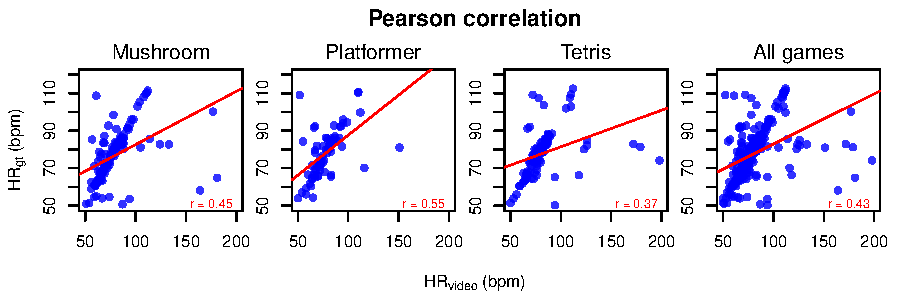
\includegraphics[width=\columnwidth]{figures/correlation-hrgt-hrvideo.pdf}
\caption{Statistical correlation of $HR_{gt}$ and $HR_{video}$ when applied to the video segments of each game, as well as to the video segments of all games.}
\label{fig:chart-r-games}
\end{figure}

To better analyze the variations regarding estimation errors among subjects, figures \ref{fig:chart-hists-me} and \ref{fig:chart-hists} show a distribution of values of $M_e$, RMSE and $M_{eRate}$ for all games combined and individually. The x-axis represents intervals of values of $M_e$, RMSE or $M_{eRate}$ while the y-axis represents the percentage of subjects that presented an estimation error within the interval informed in the x-axis.

Regarding the distribution of values of $M_e$, shown in Figure \ref{fig:chart-hists-me}, overall 66.1\% of the subjects presented estimations with $M_e$ within the interval [-5 bpm, 5 bpm]. For the remaining 33.9\% of the subjects, $M_e$ was spread within the interval [-20 bpm, 35 bpm]. On a game level, $M_e$ was within the interval [-5 bpm, 5 bpm] for 65\%, 68.4\% and 65\% of the subjects of the Mushroom, Platformer and Tetris game, respectively. The values for $M_e$ are more equally distributed for the Platformer game, which explains the lower values of $SD_e$ for that game when compared to the Mushroom and the Tetris game, which present less equally distributed values of $M_e$.

The distribution of values of RMSE, shown in Figure \ref{fig:chart-hists} in the first row, indicate that overall values were lower then 10 bpm for 59.4\% of the subjects, while the remaining of the subjects had RMSE varying from 10 bpm to 50 bpm. On a game level, RMSE was lower than 10 bpm for 50\%, 68.5\% and 60\% of the subjects of the Mushroom, Platformer and Tetris game, respectively.

Regarding $M_{eRate}$, shown in Figure \ref{fig:chart-hists} in the second row, overall 69.5\% of subjects had HR estimations that were up to 10\% different than the expected HR from ground truth. On a game level, in total 73.7\% and 70\% of the estimations performed by the rPPG technique during the Platformer and the Tetris game, respectively, presented $M_{eRate}$ interior or equal to 10\%. Those values are slightly better than the 65\% of the subjects with $M_{eRate}$ up to 10\% in the Mushroom game. Despite the fact that $M_{eRate}$ was similar for both the Platformer and Tetris games, the former presented no subjects whose $M_{eRate}$ was greater than 30\%, while the later presented 10\% of the subjects with $M_{eRate}$ greater than 30\%.

\begin{figure}[!h]
\centering
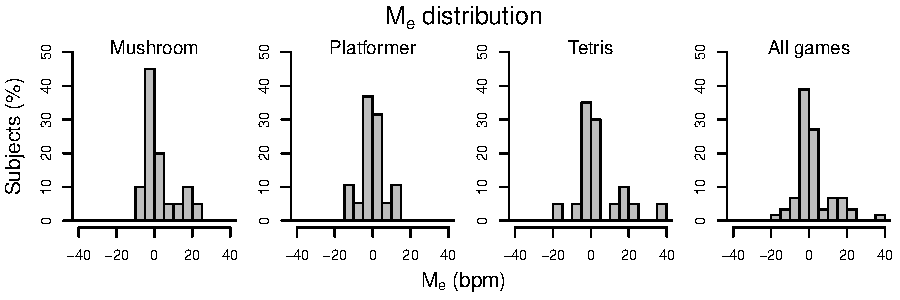
\includegraphics[width=1.0\textwidth]{figures/hist-me.pdf}
\caption{Distribution of values of $M_e$ for all games. The x-axis represents intervals of values of $M_e$ while the y-axis represents the percentage of subjects that presented an estimation error within the interval informed in the x-axis.}
\label{fig:chart-hists-me}
\end{figure}

\begin{figure}[!h]
\centering
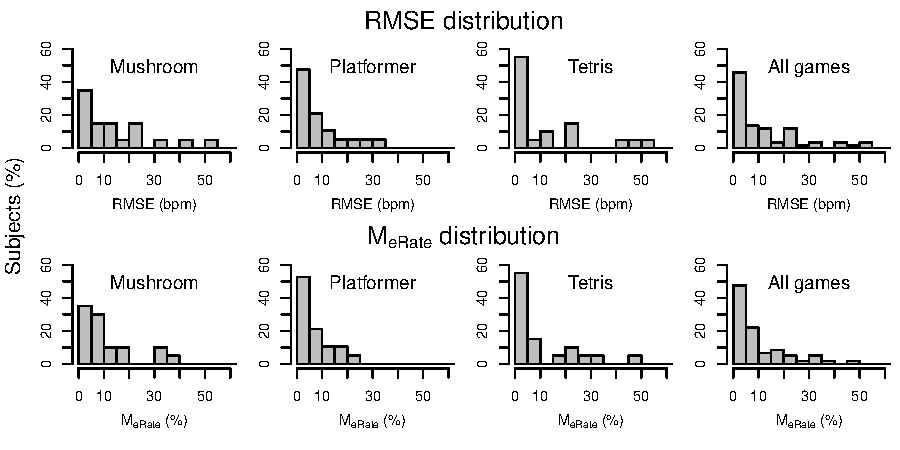
\includegraphics[width=1.0\textwidth]{figures/hist-rmse-mrate.pdf}
\caption{Distribution of values of RMSE and $M_{eRate}$ for all games. The x-axis represents intervals of values of RMSE or $M_{eRate}$ while the y-axis represents the percentage of subjects that presented an estimation error within the interval informed in the x-axis.}
\label{fig:chart-hists}
\end{figure}

\subsection{Discussion}

The results obtained indicate that the use of the selected rPPG technique to estimate HR from videos of gaming sessions is feasible. When the technique was applied to a testing set of 20 manually selected 30 seconds long video segments, whose subject's facial activity and body movement were minimal, the estimations were significantly accurate. As demonstrated by Table \ref{table:rppg-validation}, the mean of error-rate $M_{eRate}$ was 1.52\% and the Pearson's correlation coefficient was $r = 0.99$ for that testing set. Those results were expected since the videos featured an unrealistic condition where subjects remained mostly still with a neutral face.

When the rPPG technique was applied to all gaming sessions, however, body movement and facial activity significantly impacted the estimation performance. It is aligned with previously described works in the literature, which indicate the estimation error increases when subject activities increase \parencite{Wang_2016novel}.

The elevated values for $SD_e$, the standard deviation of $M_e$, suggest significant variations in the estimations among subjects in each video segment. The estimation discrepancies do not seem to be caused by errors equally spread among all gaming sessions, but due to a subset of problematic ones instead. The discrepancies and skewness of the estimations are visible in the scatter plot of the estimated and expected HR values in Figure \ref{fig:chart-r-games}. It shows a cluster of points for each game, however it is surrounded by significantly wrong estimation points. In the Mushroom game, for instance, 5 estimations (bottom right of the chart) were in the interval [120 bpm, 181 bpm] bpm, which is significantly outside the expected ground truth interval of [80 bpm, 110 bpm]. Similar significantly wrong estimations can also be seen in the Platformer and the Tetris game.

The skewed distribution of values of $M_e$, $M_{eRate}$ and RMSE illustrated in figures \ref{fig:chart-hists-me} and \ref{fig:chart-hists} also support that indication. Considering the estimations for all games, in total 69.5\% of them presented $M_{eRate}$ related to an estimation value that was less than 10\% different than the expected HR from ground truth. Additionally 59.4\% of all estimations presented RMSE lower than 10 bpm. That result is slightly worse when compared to similar works that used rPPG techniques and subjects featuring natural movements, whose reported RMSE was between 0.11 and 7.28 bpm.

A direct comparison of the results of this study to the ones of such similar works is unfair however. Despite the fact that the aforementioned works present experiments where subjects are told to behave naturally, their accuracy evaluation is based on artificial human-computer interactions, as previously described in Section \ref{s:study3}. The accuracy results of the present study account for body and facial movement caused by games whose focus is entertainment, not artificial interactions. As a consequence, the results are more connected to a scenario involving real and spontaneous reactions to games, showing that the estimations of the rPPG technique are feasible, however skewed by other factors such as natural facial activity and subject movement.

The differences in estimation also seem to be connected to the particularities of each game and subject. Considering the distribution of values of RMSE and $M_{eRate}$, both the Platformer and the Tetris games presented more estimations with lower error than the Mushroom game. The Mushroom game presented 15\% of its estimations with RMSE greater than 30 bpm and $M_{eRate}$ greater than 30\%, which are significantly wrong estimations.

In order to further explore such differences in estimations, the variations of movement and size of the ROI used to track the subject's face along the videos was analyzed. A stable ROI (both in shape and movement) is required for a precise extraction of the plethysmographic signal, so significant variations in the ROI lead to estimation errors. The mean position of the center point of the ROI for each subject in each gaming session was calculated. For each subject in each game session, the Euclidean distance between the center point of the ROI of each frame and the mean center point of the ROI previously calculated (for that subject in that session) was measured.

Similarly the mean length of the ROI diagonal for each subject in each game session was calculated, subtracting it from the length of the ROI diagonal of each frame in that gaming session. Since game sessions differ in time duration, the subject's progress in the game was normalized using the interval [0, 1], where 0 is the start point of the gaming session and 1 its end. Measurements were also subtracted from the sessions mean to facilitate analysis and comparison among different games/subjects.

\begin{figure}[!h]
\centering
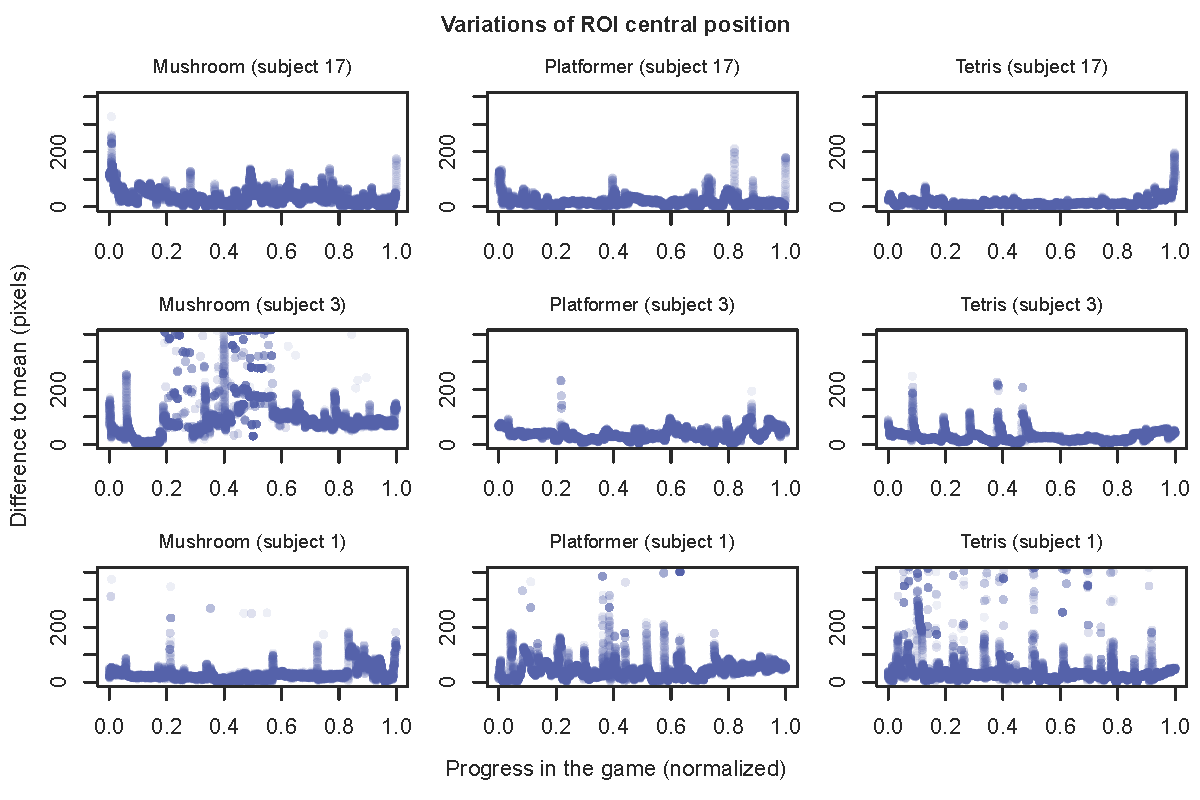
\includegraphics[width=\textwidth]{figures/variation-roi-center.png}
\caption{Variations of distance of the ROI central position for subjects 17 (low estimation errors), 3 (moderate to high estimation errors) and 1 (high estimation errors) during their gaming sessions. Values were subtracted from session mean to facilitate analysis and comparison among different games/subjects.}
\label{fig:chart-roi-anomalies-center}
\end{figure}

Figure \ref{fig:chart-roi-anomalies-center} illustrates some of the patterns observed in the investigation of the distance of the ROI central position. Each row in the figure contains three charts showing the variations of the ROI central position along the gaming sessions of a given subject. The first row contains the investigation of subject 17, who presented, for all his/her gaming sessions combined, -0.33 for $M_e$ ($SD_e$ 1.4) and 1.39 for RMSE (low estimation errors). The second row shows subject 3, who presented 11.47 for $M_e$ ($SD_e$ 16.47) and 19.62 for RMSE (moderate to high estimation errors). Finally the third row shows subject 1, who presented 15.94 for $M_e$ ($SD_e$ 28.5) and 31.96 for RMSE (high estimation errors).

The estimations performed on subject 17 were significantly accurate and the charts regarding the variation of the ROI central position show a stable progression along all gaming sessions. The distance variation (y-axis) remains mostly concentrated within the interval of [0, 100] pixels for all games, which suggest the subject presented few or short movements during gaming sessions. Subject 3 also presented low variation in the Platformer and the Tetris game, however there is a significant variation in the ROI central position in the Mushroom gaming session. The chart indicates significant distance variations of the ROI that are above 200 pixels in a certain period of the game. Finally subject 1 presents high variations in the ROI distance in all gaming sessions, as demonstrated by points above the 200 pixels mark regarding the difference to mean. The Tetris game, in special, present distance variations above 200 pixels during almost the whole session.

\begin{figure}[!h]
\centering
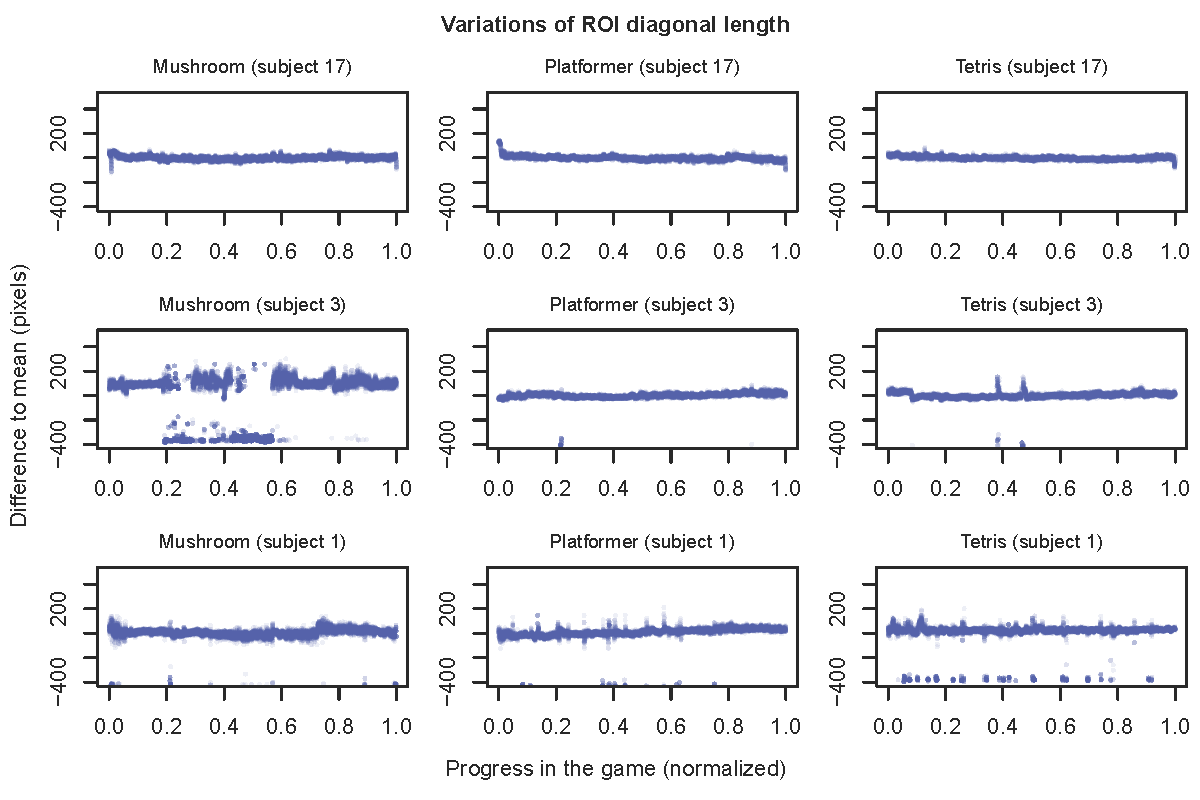
\includegraphics[width=\textwidth]{figures/variation-roi-diagonal.png}
\caption{Variations of ROI diagonal length for subjects 17 (low estimation errors), 3 (moderate to high estimation errors) and 1 (high estimation errors) during their gaming sessions. Values were subtracted from session mean to facilitate analysis and comparison among different games/subjects.}
\label{fig:chart-roi-anomalies-diagonal}
\end{figure}

Figure \ref{fig:chart-roi-anomalies-diagonal} illustrates the same subjects regarding the investigation of the variations of the ROI diagonal length. Similarly to the variations of the ROI central position, the variation of the ROI diagonal length (y-axis) is lower for subject 17 (first row of charts in the figure), since the majority of the values are close to zero. Subject 3 also presents low variations in the ROI diagonal length during the Platformer and the Tetris game, however there are significant changes in the ROI size during a period in the Mushroom game. In such period, the length of the ROI diagonal is negative, i.e. -400 pixels, which indicates the size of the detected ROIs for those frames was smaller than the mean ROI diagonal length. It could be caused by a wrongly detected face (false-negative), for instance. Finally subject 1 presents, to some extent, variations of the ROI diagonal length during the majority of his/her gaming sessions. Those constant variations could be caused by the inability of the face tracking algorithm to stably and continuously detect the subjects face along the frames of the video. The chart shows a distribution of values along the zero mark regarding difference to mean, however they are more spread than those of subject 17, for instance, which indicates higher instability of the ROI size/detection for subject 1. In the Tetris session of subject 1, for instance, there are extreme variation in the ROI diagonal length with values close to -400 pixels, similarly to the ones of subject 3 in the Mushroom game. Such extreme variation could also be explained by a wrongly detected face area during those frames.

An inspection of the videos of subjects with patterns similar to the ones of subjects 3 and 1 revealed sensitive amount of movement and facial activity, including occlusion of the face by the subject's hand, as illustrated by Figure \ref{fig:face-variation}. Any facial occlusion influences the face tracking algorithm used (Viola\&Jones), since it might wrongly detect the face position or do not detect it at all. A flawed face detection step affects the extraction of the plethysmographic signal, because noise is extracted along with the raw signal, making the rPPG technique unable to separate it properly.

Despite the efforts to create games that prevented face occlusion by the subject's hand, such behavior seems to be natural in boring situations. Both Mushroom and Tetris games were more likely to allow players to place a hand in the face to express boredom, since the games could still be played with a single hand when the gameplay speed was not elevated. The Platformer game, on the other hand, is less likely to allow players to use only a single hand to play, which reduced chances of face oclusion inferering with the face tracking algorithm. This could also explain why estimations made during the Platformer game were more accurate than those performed during the other two games. Those extreme cases with facial occlusion are probably affecting the error rates in the analysis, producing less accurate estimations. Such extreme and flawed cases could have removed from the analysis, however the aim is to test how the selected rPPG technique performs in natural gaming situations. A dataset with untreated videos of gaming sessions with natural interactions might produce sub-optimal HR estimations, however it is the understanding that stressing the rPPG technique with less artificial videos provides researchers with insights about possible problems and accuracy limits of such tool.

\begin{figure}
\centering
  \begin{subfigure}[b]{0.5\textwidth}
    
\includegraphics[width=0.95\textwidth]{figures/face-occlusion}
    \caption{}
    \label{fig:face-occlusion}
  \end{subfigure}%
  \begin{subfigure}[b]{0.5\textwidth}
    \centering
    
\includegraphics[width=0.95\textwidth]{figures/head-tilt}
    \caption{}
    \label{fig:head-tilt}
  \end{subfigure}
  \caption{Examples of body movement and facial activity during gaming sessions. (a) Partial face occlusion by subject's hand; (b) Head tilt and movement during laugh action.}
  \label{fig:face-variation}
\end{figure}

It is possible to speculate that the variations regarding movement and size of the ROI, which directly influence estimation accuracy of the rPPG technique, seem to be connected to the unique behavior of each user as well. As illustrated by Figures \ref{fig:chart-roi-anomalies-center} and \ref{fig:chart-roi-anomalies-diagonal}, subjects present different movement patterns. Previous analysis of the videos indicates significant differences regarding facial activities among subjects \parencite{bevilacqua2016variations}. It strengthens the idea of a user-tailored model able to deal with such peculiarities, which is more likely to produce better estimations. A method that operates its estimations based on the average user behavior is prone to be significantly affected by specific user behavior outside the expected mean pattern, causing skewed distribution of estimation errors such as the ones presented on Figure \ref{fig:chart-hists} regarding $M_{eRate}$ and RMSE.

%\subsection{Limitations}

%Some limitations of the experimental procedure and analysis should be noted. The 1-minute long duration of each video segment used for the estimation of HR may affect the results. The ideal length of the video segment used for estimation (called window size) is not agreed upon in the literature \parencite{rouast2016remote}. In general, it depends on the characteristics of the rPPG technique being applied as well as the hardware configuration, such as camera framerate \parencite{roald2013estimation}. We selected a 1 min analysis window based on the information of the original work by \textcite{poh2011advancements}. Additionally our experimental procedure consists of games whose difficulty level changes every 1 minute, so that value is aligned with the window size used for HR estimation. As previously described, the statistical nature of ICA, part of the selected rPPG employed in the experiment, demands longer video samples to produce accurate results. The longer the video, however, the higher the chances of subject motion, which increases noise. A trade-off between the duration of the video segments and the estimation accuracy could be better investigated. Our experimental setup used an external light source to minimize noise caused by changes in illumination, which should narrow the estimation error to causes as subject movement and/or facial activity. It is likely, however, that other factors might impact the estimation accuracy, such as facial hair, e.g. beard and hair over the forehead area, use of glasses, and skin color.

\subsection{Conclusions}

Overall the estimation of the rPPG was feasible, showing mean estimation error of 2.99 bpm (SD 18.83 bpm), RMSE of 19.03 bpm and a positive and medium strength Pearson correlation of $r=0.43$, $p < 0.001$. On average, the estimation error of the rPPG technique was up to 10.31\% of the expected value calculated from ground truth. Additionally the exploratory investigation regarding factors that impacted the accuracy of the rPPG technique, such as variations in the region of interest (ROI) used to remotely extract the HR signal, suggest factors connected to the type of the game being played and the unique behavior of each subject influenced the estimations. Among the causes of such influence were identified body movement, e.g. head tilt and rotation, and facial occlusion by subjects hand.

%Our results provide researchers with information related to the reliability of a remote HR measurement technique when applied to the context of games research. We believe our experimental setup is a novel approach in the exploration of the accuracy of rPPG-estimated HR readings of subjects in a gaming context. To the best of our knowledge, our experiment is the first to measure the accuracy of an rPPG technique with the use of three boredom/stress-inducing games with subjects behaving naturally. Future work involves investigation of facial activity as well as body movement as a complementary source of information to be used along with remote HR estimation in a multimodal analysis for the identification of stress and boredom in games. As demonstrated, subject movement affects rPPG estimations, however it is an inherent characteristic of a gaming session with natural behavior. We will analyse the use of such signals in a user-tailored approach, focusing on the particular behavior of each user instead of the average pattern.

